\section{Problem definition}\label{sec:problem_definition}

Social Networks (SN) are a powerful tool for understanding complex social systems, in which relationships between actors play a central role. Because of this, Social Network Analysis has become increasingly popular in the Political Science community for studying the dynamics of power. For instance, the authors of \cite{fowler2006connecting} studied a graph of co-sponsorship of bills to study interactions between congressmen in the US House of Representatives and found that by using network analysis tools it was possible to find highly influential politicians. Similarly, in \cite{kirkland2011relational} the authors  developed a theory of influence diffusion across a legislative network of relations based on weak and strong links and found patterns useful for determining the success of a bill.\\

The growing popularity of SNA in Politicial Science has given birth to Policy Network Analysis, a discipline concerned in the creation and analysis of SN involving political actors.\\

%In \cite{thomas2006get} we find a proposal to predict the voting of a bill based on speeches made by congressmen by detecting evidence of endorsements.  \\

\subsection{Policy Networks: Social Network Analysis for Political Science}\label{subsec:defining_pn}

\emph{Policy Network Analysis} (PNA) is the discipline in Political Science which focuses on the discovery and analysis of links between government and other members of a society, with a particular interest in the understanding of the policy making process and its outcomes. There are plenty of definitions of Policy Networks (PN) in the literature, basically because there are many ways to characterize relationships between actors of a society and several ways to approach the analysis. However the Oxford Handbook of Public Policy proposed a definition which is widely accepted and encompasses many of the other proposals. They state that a PN is a ``set of formal institutional and informal linkages between governmental and other actors structured around shared if endlessly negotiated beliefs and interests in public policy making and implementation''\cite{moran2008oxford}. \\

One of the main difficulties in PNA is that the generation of these PN is usually done in manual, cumbersome processes by experts. This involves the use of interviews, questionnaires and other instruments from the social sciences. During the actual generation of the network many subjective factors may come into play as the overall result depends on the people involved in the study. Consequently, PN generation involves a significant investment that does not always ``lead to breathe taking empirical and theoretical results'' \cite{kenis1991policy}. The question is consequently, how can we use technology to improve the process of PN identification. 

\subsection{Towards the automatic generation of PNs: defining our objectives}\label{subsec:objectives}

The main objective of this study is to propose a method for the automatic generation of PN surrounding the Legislative Branch of government. We decided to focus on the Legistative Power for two reasons. First, as we have previously established, Parliaments write laws and regulations, and thus have an enormous power in the shaping of a society. This makes them the primary target of lobbyists. \\ 

Second, as we will later see in section \ref{sec:related-works}, the challenges of automatic Social Network generation lie in i) understanding and characterizing the links found among the actors occurring in the SN and ii) discovering hidden relationships, which can only be detected by learning that two entities share a common topic.  When outlining this study, we aimed to define the problem in a way that we could address these two difficulties and produce SN which are meaningful, easy to interpret and with the highest number of possible relevant connections. \\

As we will see later on, bills can then be used as a cornerstone for detecting relationships between politicians and third-party actors. \\% We show that given a law it is possible to i) track the participation and the position of a politician with respect to it, ii) find entities in news articles which could be directly related to its content, iii) compute similarity measures between entities - and generate a graph - by taking into account their relationship to the bill iv) use the bill to label the discovered relationships.\\

The reader should know that for the rest of this document, we use the words bills and laws exchangeably to refer to the rules and regulations approved by a legislative body. We also use the terms entity, actors, political actors to refer to companies, non-governmental organizations, governments, advocacy groups, citizens and in general any person or association that is related to a bill, meaning that the contents of the bill affect their interests or policies. \\

\subsection{What type of PN do we aim to generate?}\label{subsec:objectives}

Among the different types of PN that we could study, we are concerned with the generation of two types of SN, or graphs. First, we are interested in generating SNs depicting the relationship of relevant actors with the bills approved by a legislative body. This SN, which we will call the \emph{Bill-Entity graph} is a di-graph with two types of nodes: bills and entities. In the \emph{Bill-Entity graph} graph there is a link between a bill and an entity if and only if the entity is related to the bill. This type of graph is useful for understanding how different actors relate to the bills, and for also understanding how the latter are interrelated.\\

Second, we are interested in generating, from the \emph{Bill-Entity graph}, an \emph{Entity-Entity graph} capturing possible relationships between two actors. These definition of this type of relationship is vague: we are interested in discovering pairs of actors that are i) related to a bill and ii) are politically affine or antagonistic, meaning that they could possibly know each other, be in contact and cooperate or compete to push their agendas. \\  

In many cases entities have either a positive or negative position with respect to a law. In the case of politicians, their voting history for a particular bill is recorded and usually accessible through Parliament websites or open data. In the case of companies, NGOs and other types of actors, their position could be assessed automatically, by employing sentiment analysis or other NLP techniques, or manually by experts. \\ 

This polarity can be used to annotate the links of the \emph{Bill-Entity graph} and the relationships of the \emph{Entity-Entity graph} by the following premise: two entities are positively related if they are positively or negatively related to a common bill; similarly, two entities are negatively related if they have different polarities with respect to a common bill. Naturally it might be the case that an actor does not have a well-defined relationship with respect to a law or that it is impossible to objectively classify it. Nonetheless, this schema allows for the generation of enriched graphs which allow for more refined graph analysis techniques. For instance, in \cite{traag2009community} we find a community detection algorithm which works with positive and negative links. 

\subsection{Stop Online Piracy Act (SOPA): a motivating example}\label{subsec:objectives}

\begin{figure}[h!]
    \centering
    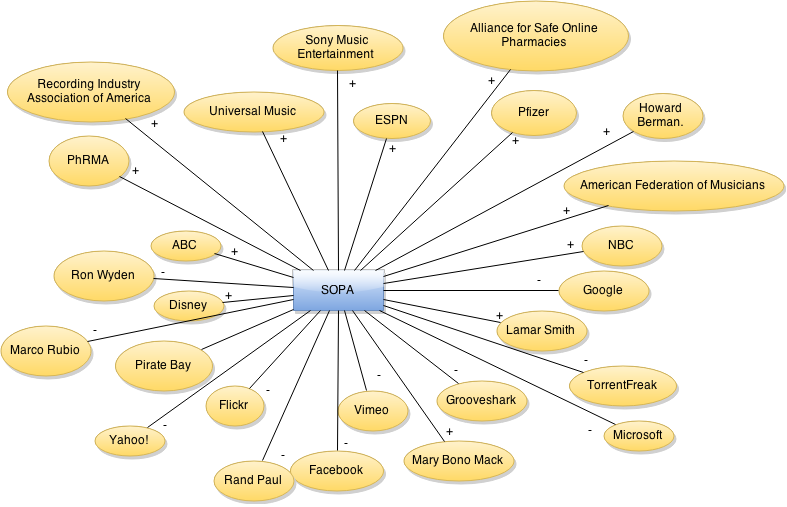
\includegraphics[width=1\textwidth]{figs/sopa_bill_entity.png}
    \caption{Bill-entity graph for SOPA.}
    \label{fig:example_bill_entity}
\end{figure}

\begin{figure}[h!]
    \centering
    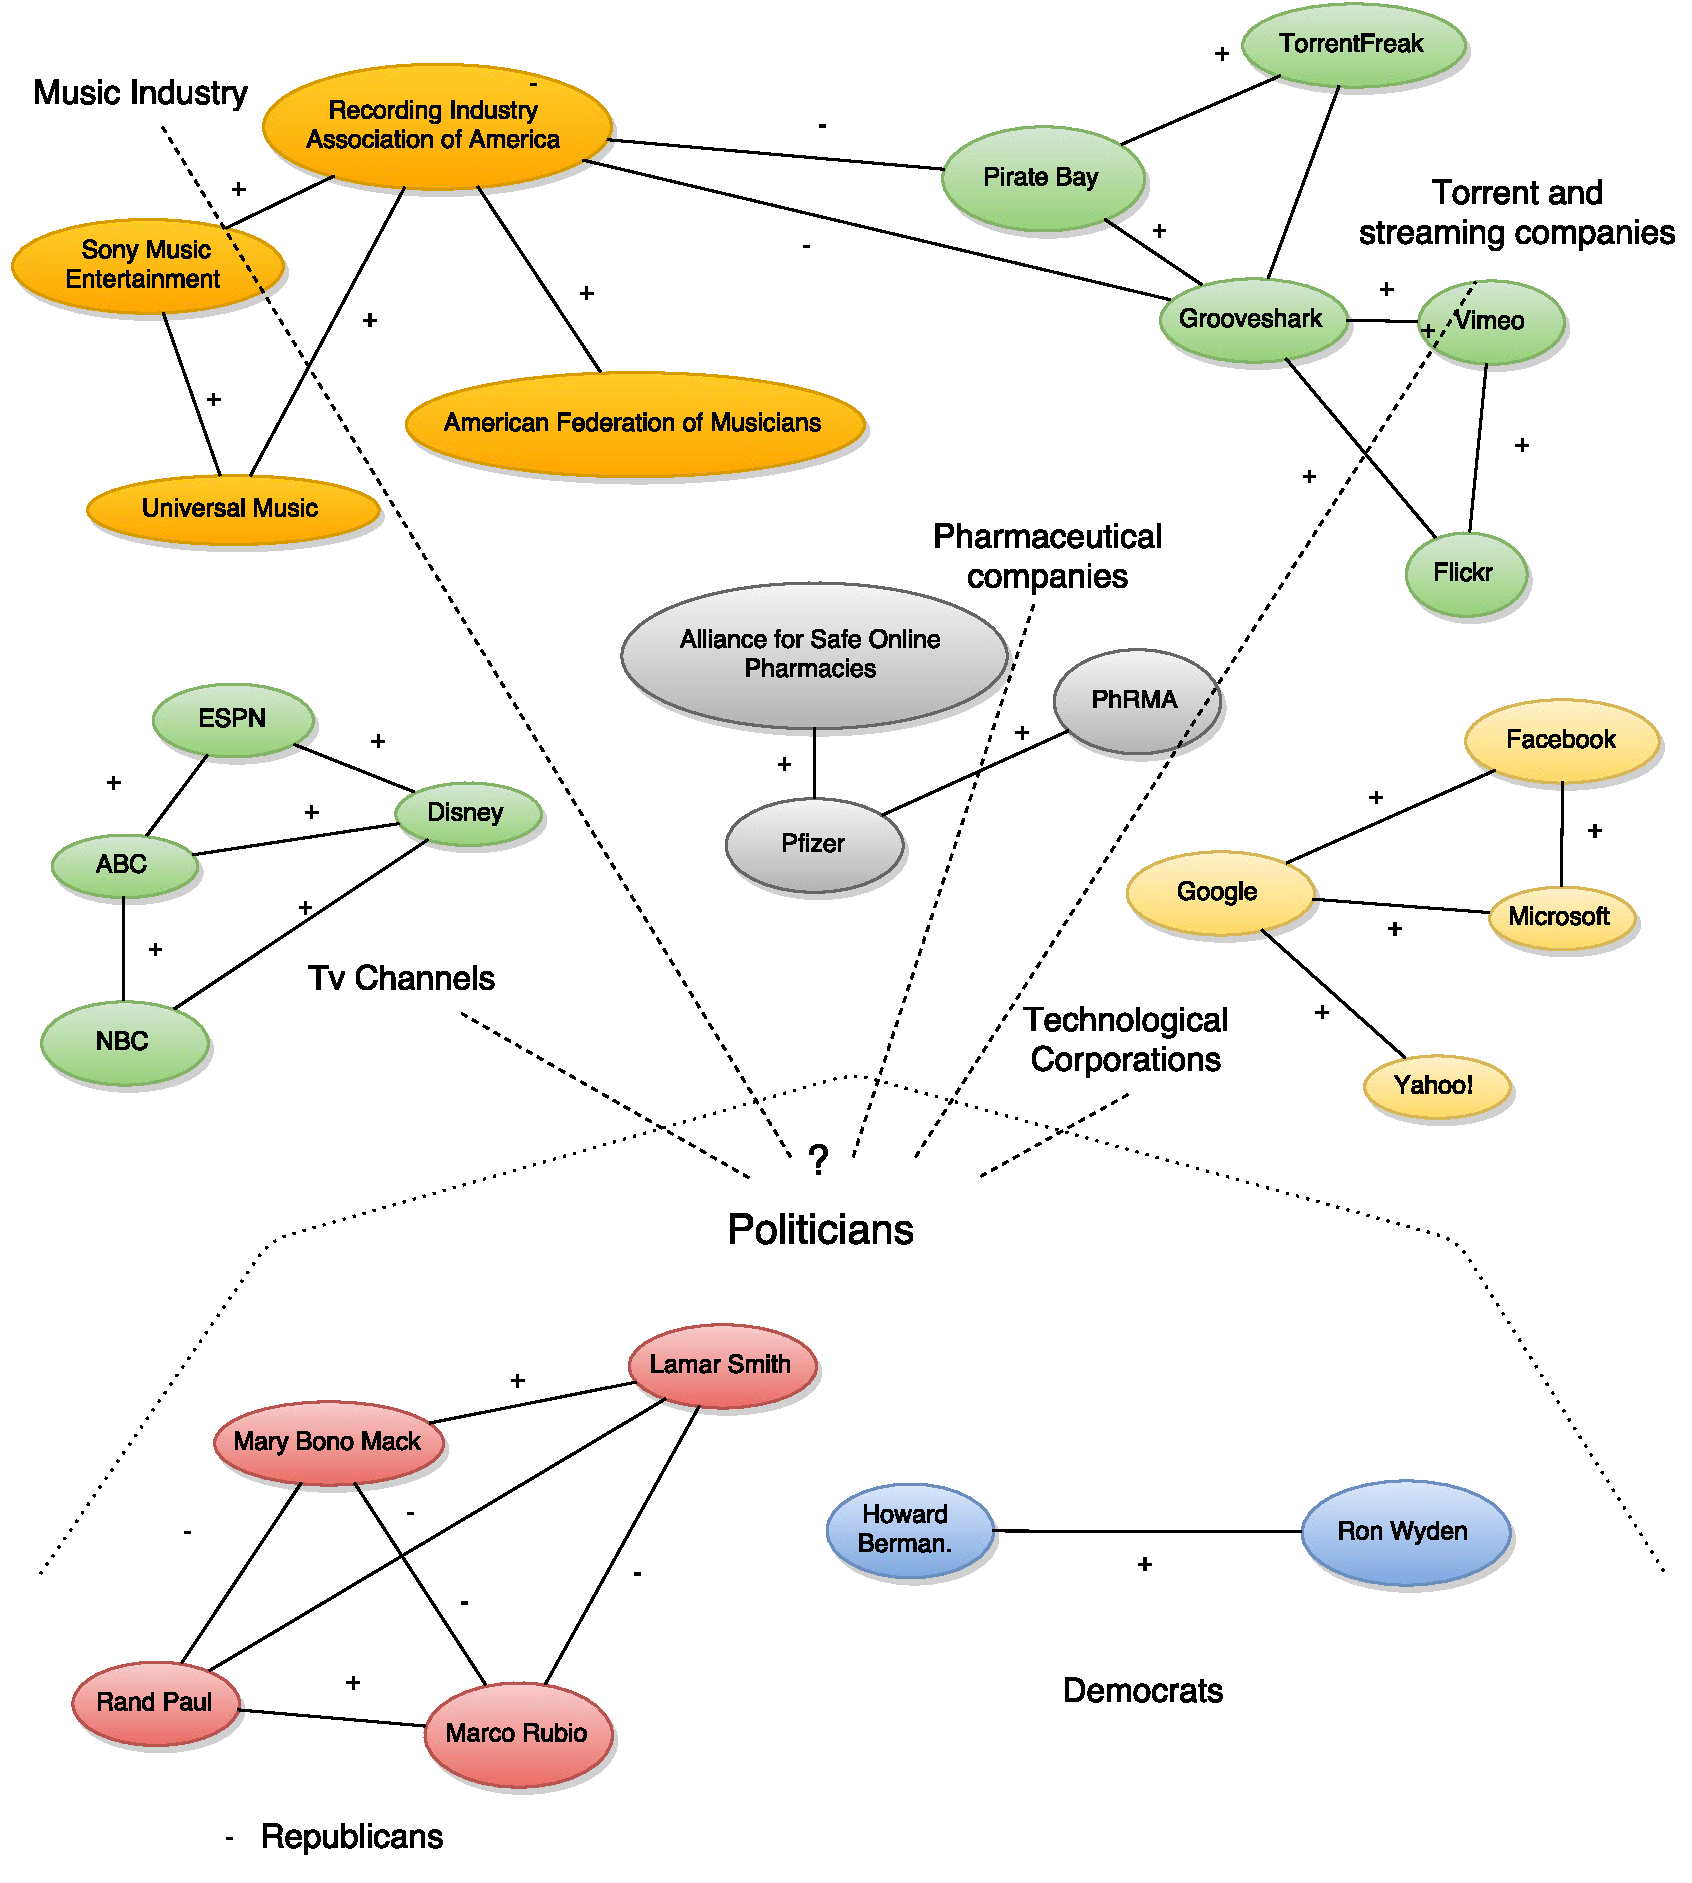
\includegraphics[width=1\textwidth]{figs/sopa_entity_entity.png}
    \caption{Entity-entity graph for SOPA.}
    \label{fig:example_entity_entity}
\end{figure}

As an illustrative  example, consider the \emph{Stop Online Piracy Act} (SOPA). SOPA was a bill introduced in 2011 the United States to combat online copyright infringement and online trafficking in counterfeit goods. If a website was found to infringe the law, SOPA allowed court orders to require Internet service providers to block access, prevent search engines from listing them and forbid advertising networks or other payment facilities from conducting business with the website. SOPA also made the unauthorized streaming of copyrighted content a criminal offense, imposing a penalty of up to five years in prison. \\ 

Due to it's controversy, SOPA was widely discussed internationally and many organizations raised their voices in favor and against the bill\footnote{A list of organization in favour and against can be found in \url{http://en.wikipedia.org/wiki/List_of_organizations_with_official_stances_on_the_SOPA_and_PIPA}}. In broad terms, organizations which rely on copyright strongly supported the bill. This includes, for instance:

\begin{itemize}
\item {\bf Pharmaceutical companies and associations}  like Pharmaceutical Research and Manufacturers of America (PhRMA), Pfizer, Alliance for Safe Online Pharmacies (ASOP). 
\item {\bf TV channels}: ABC, NBC, ESPN, Disney, among others. 
\item {\bf The music industry}, including the Recording Industry Association of America, the American Federation of Musicians, Sony Music Entertainment, Universal Music, etc.
\end{itemize}

Similarly, organizations that advocate for freedom and liberties, or whose business would be negatively affected by increased regulations voiced the opposition against the bill. Among these, we highlight:

\begin{itemize}
\item {\bf Torrent and streaming companies}: such as Pirate Bay, TorrentFreak, Vimeo, Grooveshark, Flickr, etc
\item {\bf Technological corporations}, such as Facebook, Yahoo!, Microsoft, Google.
\end{itemize}

Finally, we can also know the position of congressmen by looking at their voting history or their positions. In the case of SOPA, Republicans Lamar Smith and Mary Bono Mack, and Democrat Howard Berman were among the sponsors of the bill, while Democrat Ron Wyden and Republicans Marco Rubio, Rand Paul were against.\\

Based on this information, which we have manually gathered, we could generate a \emph{Bill-Entity graph} and an \emph{Entity-Entity graph} as the ones shown in figures \ref{fig:example_bill_entity} and \ref{fig:example_entity_entity}. These graphs were generated in a manual way taking into account the relationship of the entity with respect to the bill as defined before. \\

Note that the \emph{Bill-Entity graph} is not particularly useful by itself as it is only a way to visualize the information about a specific law. However if analyzed along with other bills, we can see how they overlap and understand for instance the similarity between two bills based on the entities that are related to them, the distance between two actors based on the whole set of legislations, compute centrality measures to detect influential politicians, etcetera. \\ 

The \emph{Entity-Entity graph} is useful on another hand for detecting communities of actors that share similar interests for a specific bill. Note that we deliberately chose not to draw edges between the politicians and the rest of the political actors; this is because we do not have the knowledge to suggest that a politician and a company might be related. We decided to draw only links between organizations of the same type, with the exception of the relationship between the Recording Industry Association of America and Grooveshark, TorrentFreak and PirateBay. Since the latter three are used to illegally download music we can infer that they are related. Our objective in this study is to produce a system that can automatically detect these and other obscure relationships automatically. \\

What type of analysis can we do with the \emph{Entity-Entity graph}? We can use the traditional SNA tools to individually analyze bills or alternatively look at the overlapping of these graphs accross different bills. This graph is however particularly useful for detecting possible lobbying relationships. For instance if a politician (or group of politicians) has a high number of links with the political actors of a specific community (imagine for instance that Lamar Smith had links with most of the Music Industry group) then we could possibly infer that there is a lobbying relationship.  \\


\subsection{Is it really possible to detect lobbying in an automated way? An important caveat}\label{subsec:really_lobbying} 

It is important to clarify that despite being motivated by the detection of patterns that can be suggestive of a lobbying process, in practice we aim to find relationships of political similarity or dissimilarity between two entities. The relations found by our method do not necessarily imply that the two actors are in direct liaison;  to do so we would need to closely monitor all the activities of politicians and organizations to verify with whom they are in contact. This is naturally unreasonable due to privacy considerations. \\

We aim to detect links between entities that indicate that they are both related to a particular political decision - in our case bills -, from which we could then establish political affinity or aversion. Naturally, if two entities have highly similar political views in a broad set of issues then one can believe that they could be collaborating. This could be verified by investigative journalists and by considering other sources of information like donations information, speeches, etcetera. Regardless of the verification of a lobbying process, our method is intended to be an unbiased, low-cost, semiautomated toal to aid the process of Policy Network generation and analysis. 

